\begin{chaptercover}{Scope}%
{\coverepigraph{``Drones cause problems for more and more types of secure sites, whether it’s a matter of irresponsible or nefarious operators […] taking photos where you shouldn’t be taking photos or putting people on the ground at risk."}{\textsc{Nimo Shkedy} \newline {\normalsize\vspace{-.3cm}CEO of ApolloShield}}
{\large \hyphenation{} \bigletter{}{} {\color{red} ...}\newline\\}}%
{scope}

Now that we have set the basics of what is penetration testing, we can move to the actual application of the concept to the drones. 

The first phase of the work consists in gathering as much information as possible regarding the current state-of-the-art on drone security.

\section{Literature review}

This section focuses on showing a possible design of a drone and a compilation of security-relevant information. As part of that effort, the following emphasizes on giving a ready reference of one particular vulnerable drone and associated open source attack tools that have already been developed. This compilation should provide the reader with a better understanding of how drone vulnerability is currently exploited, and how future drone will take advantage of improvements in available vulnerability research data.

\subsection{Typical drone design}\label{subsec:typical-drone-design}

In every model of light commercial drone, we can figure out that a pattern always appears with the components as depicted in Figure \ref{fig:drone-design}.

\begin{figure}[H]
  \centering
  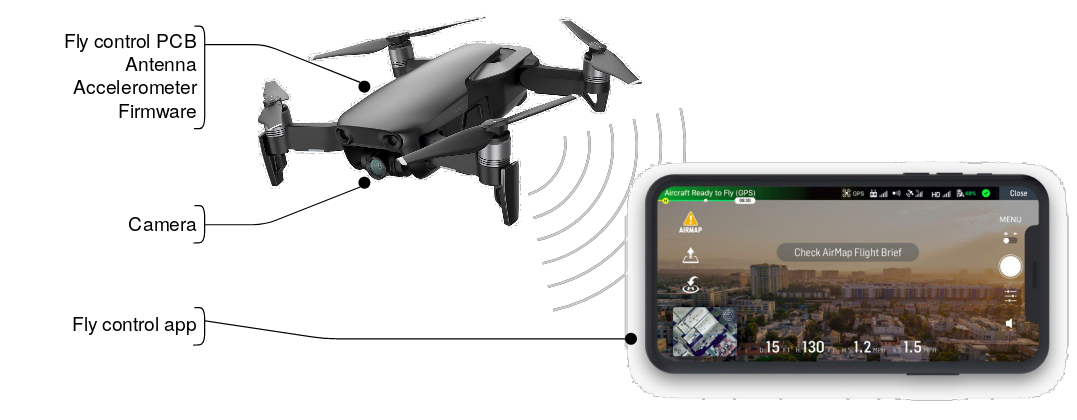
\includegraphics[width=\linewidth]{figures/drone-design}
  \caption{Typical design of a light commercial drone and its remote control}
  \label{fig:drone-design}
\end{figure}

\begin{itemize}
  \item \textbf{Fly control PCB} : It contains a microcontroller for holding drone's software.
  \item \textbf{Antenna} : Depending on the wireless techonology, lots of drones hold a WiFi antenna in 2.4GHz.
  \item \textbf{Accelerometer} : This is required for the stabilitization of the drone.
  \item \textbf{Firmware} : This can be a light Unix-based ARM operating system like HiLinux \cite{hilinux} with a toolkit like BusyBox \cite{busybox}. Sometimes, an update mechanism can be used, e.g. through FTP for the transfer between the remote control and the drone.
  \item \textbf{Camera} : This streams the filmed images through a protocol like \acrshort{rtsp} \cite{rfc7826}.
  \item \textbf{Fly control application} : When using a smartphone as the remote control, this can be an Android or iOS application.
\end{itemize}

In the case of WiFi drones, these act as the \acrfull{ap} to the remote control, embedding a WiFi module in the \textit{Fly control PCB}.

\subsection{Parrot AR Drone}

\begin{center}
\begin{tabular}{m{5cm}m{12.3cm}}
\hyphenation{produced}
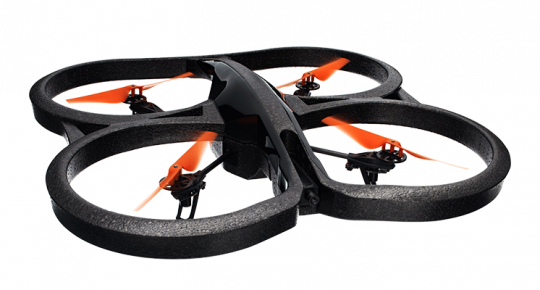
\includegraphics[width=\linewidth]{parrot-ar-drone-2} & The Parrot AR Drone 2.0 is one of the most popular quadcopters produced. This is a cheap drone that is both quick and fast. It is controlled by an iOS or Android smartphone or tablet and allows 720p live high-definition video streaming and recording in flight. \\
\end{tabular}
\end{center}

This device is a good reference on how one of the most popular commercial drones totally lacks security. Security breaches are numerous, let’s review them :
\begin{itemize}
  \item \textbf{Open FTP on port TCP/21} : Simply just connect to the IP without any username or password, and have access to the directory of the drone, where it stores the recorded videos.
  \item \textbf{Open Telnet on port TCP/23} : Once again, simply just connect to the IP without any username or password, and you are logged in. Furthermore, it's running Linux and it is a root access to the device! At this point the attacker could simply issue a shutdown and watch the drone fall to the ground.
  \item \textbf{Unencrypted communications} : A simple capture of the communication packets between the drone and the controller allows the attacker to have an easy view of the protocol. Once he has successfully analyzed the main commands, he can easily replay them -- for example using the python Scapy library -- in order to hijack the drone.
  \item \textbf{WiFi controlled} : The drone is controlled with an app through WiFi, and by default, it isn’t even password-protected ! This allows any user running the application to control the drone. Even though a security can be enabled, called \textit{Pairing}, which will make the drone drop the packets if the MAC address sending them is not the one it is paired with. It is nonetheless easy for the attacker to spoof the source MAC on the packets.
\end{itemize}

More information can be found on the subject at \cite{github-drone-hacking} as well as some investigations for improving the security at \cite{hacking-securing-ardrone2}.

\subsection{Known vulnerabilities}

As defined in Subsection \ref{subsec:vuln-vs-weakness}, \acrshort{cve}'s are identifiers for publicly known vulnerabilities. It is therefore useful, prior to starting any pentest on drones, to look for eventual known vulnerabilities on the field. In the same way, CVE may be used once a certain service is identified on a device.

As for now, only one entry is available and concerns the DBPOWER U818A WIFI quadcopter drone :
\begin{indentbox}{1cm}
  \textbf{CVE-2017-3209} : \textit{The quadcopter drone provides \textbf{FTP} access over its own local access point, and allows full file permissions to the anonymous user. The DBPower U818A WIFI quadcopter drone runs an FTP server that by default \textbf{allows anonymous access without a password}, and provides full filesystem read/write permissions to the anonymous user. A remote user within range of the open access point on the drone may utilize the anonymous user of the FTP server to read arbitrary files, such as images and video recorded by the device, or to replace system files such as /etc/shadow to gain further access to the device. Furthermore, the DBPOWER U818A WIFI quadcopter drone uses BusyBox 1.20.2, which was released in 2012, and may be vulnerable to other known BusyBox vulnerabilities.}
\end{indentbox}

It goes without saying that a single result is terribly weak, for example, we get nearly 1,500 results just for the Apache web server (as August 2019). This tends to show that a substantive work remains to be done in this area, but also that the door is open for real progress.

\section{Scope definition}

This section presents some models of drones selected for the study and the beginning of the application of the penetration testing methodology, that is, the \textit{intelligence gathering}.

\subsection{Scope limitation}

The drones were provided by the professional supervisor within the limits of his allocated budget to cover a small spectrum of drone-related technologies in order to establish the basis of a framework (as it is explained in Chapter \ref{framework}). For a question of scope, only a few models are selected to match some technical specifications as we focus on wireless penetration testing.

For this work, we received the following six different drones. Each of them comes from a different brand so that we can cover the wider spectrum of technologies possible.
\begin{itemize}[itemsep=.1cm,topsep=.1cm]
  \item Drone S9
  \item Jamara Skip 3D Quadrocopter
  \item NINCOAIR QUADRONE MINI
  \item UdiR/C Free Loop U27 
  \item Flitt Selfie Cam
  \item C-me 1080P WiFi FPV GPS Selfie Drone
\end{itemize}

In the initial problem statement, it was decided to develop plugins for at least 3 different popular commercial drones on the framework according to the exploits that could be discovered. Rather quickly, we excluded the first four since they were not WiFi- but radio-controlled and should require the use of a different technology than the one aimed in this work. It leaved us with the last two.

\subsection{Flitt Selfie Cam}\label{subsec:flitt-selfie-cam}

Technical specifications :
\begin{itemize}[itemsep=.1cm,topsep=.1cm]
  \item \textbf{Type} : pocket-sized selfie drone
  \item \textbf{Camera} : CMOS that can record 720p video at 30 fps and shoot 1.3MP photos
  \item \textbf{Communication technology} : WiFi 2.4GHz
  \item \textbf{Control plaftorm} : Android or iOS
  \item \textbf{Documentation} : Instruction manual \cite{flitt-selfie-cam}
\end{itemize}

\begin{figure}[H]
  \begin{tabular}{m{5cm}m{12.3cm}}
  \centering
  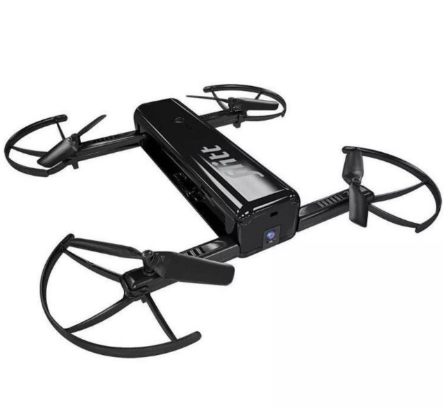
\includegraphics[width=\linewidth]{figures/flitt-selfie-cam} &
  \centering
  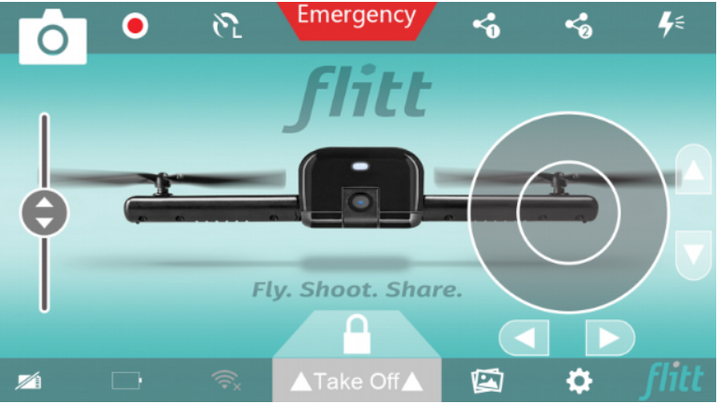
\includegraphics[width=0.63\linewidth]{figures/flitt-selfie-cam-ui} \\
  \end{tabular}
  \caption{Overview of the Flitt Selfie Cam}
  \label{fig:flitt-selfie-cam}
\end{figure}

The device can take pictures and video, adjust camera pitch, change the photo mode, and more. It must be unlocked in order to take off, auto-regulates its high and has an emergency landing feature in case of loss of control.

\subsection{C-me Selfie Drone}\label{subsec:cme-selfie-drone}

Technical specifications :
\begin{itemize}[itemsep=.1cm,topsep=.1cm]
  \item \textbf{Type} : purse-sized selfie drone
  \item \textbf{Camera} : 8MP HD 1080p camera
  \item \textbf{Communication technology} : WiFi 2.4GHz
  \item \textbf{Control plaftorm} : Android or iOS
  \item \textbf{Documentation} : Quickstart guide \cite{cme-selfie-drone}
\end{itemize}

\begin{figure}[H]
  \begin{tabular}{m{5cm}m{12.3cm}}
  \centering
  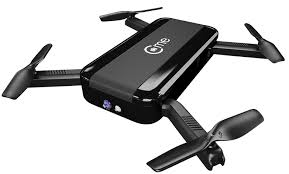
\includegraphics[width=\linewidth]{figures/cme-selfie-drone} &
  \centering
  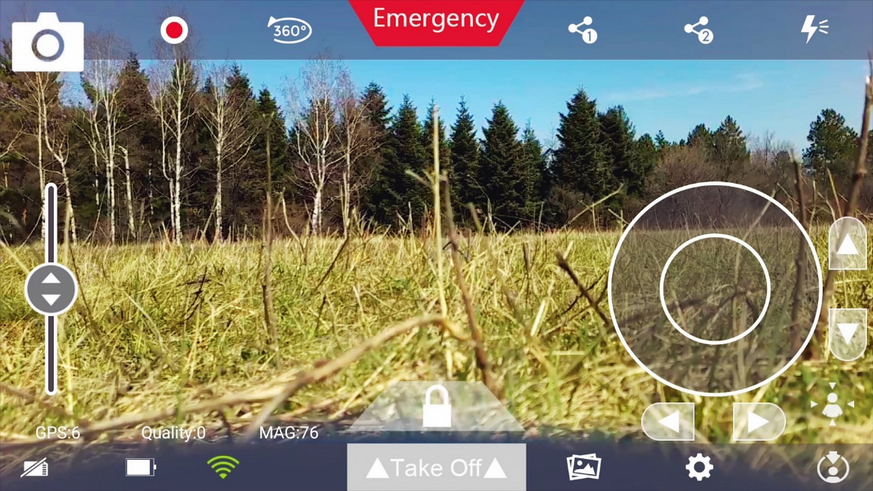
\includegraphics[width=0.65\linewidth]{figures/cme-selfie-drone-ui} \\
  \end{tabular}
  \caption{Overview of the C-me Selfie Drone}
  \label{fig:flitt-selfie-cam}
\end{figure}

The device can take high-quality pictures and video. Like the Flitt, it must also be unlocked in order to take off, auto-regulates its high and has an emergency landing feature in case of loss of control.

\begin{tip}
It is quite obvious that the interfaces are quite similar, and after further research, it turns out that the two drones are produced by the same manufacturer, i.e. Hobbico. This means that there will probably be similarities between the two devices, even though the C-me has more functionalities since it’s a little bit more expensive than the Flitt (depending on the reseller, in the 150\euro range versus 80\euro). This will be a good occasion to compare them and see if one is more secure than the other.
\end{tip}

\begin{info}
Hobbico, Inc. was a manufacturer and distributor of hobby products including radio control airplanes, boats, cars, helicopters and drones. Unfortunately, on 2018, it was announced that Hobbico had filed for Chapter 7 bankruptcy and went into liquidation \cite{hobbico-liquidation}, and the company was later bought by Horizon Hobby \cite{horizon-hobby}. There website, hobbico.com, is no longer available online and there is no reference to any of the drones on the Horizon Hobby website meaning that there is no support anymore for them.
\end{info}

\subsection{Intelligence gathering}

Given the data collected in Subsections \ref{subsec:flitt-selfie-cam} and \ref{subsec:cme-selfie-drone}, we can already find some interesting information in the provided manuals. We can figure out that both documentations mention the SSID format and the default password, "\texttt{12345678}".

Searching further for other information and documentation on search engines does not provide more data. In both cases, there is no official sales platform, so the drones are only available for sale or via third-party resellers. In these circumstances, the only information available was technical characteristics presented in ways that promote device marketing. Similarly, the posts on drone-related forums corresponding to the models we were interested in never discussed security topics, but were generally devoted to describing the control characteristics and the quality of the camera.

We then started to dismantle the drones so we could take a look at the different components. Only the Flitt could be dismantled completely without taking too much risk of damaging it. This allowed us to highlight the different components as presented in Subsection \ref{subsec:typical-drone-design}.

Even if this operation takes us out of the traditional framework of a pentest, it has allowed us to highlight an element that will eventually prove to be decisive: the Flitt uses a Hi3518 chip, but we will get back on that later.

\section{Vulnerability analysis}

The next step is to inventory the vulnerabilities on the devices. To do this, we must perform more intrusive tests than in the previous section.

\begin{tip}
First of all, it is worthwhile to mention that both drones communicate through 2.4 GHz WiFi secured with a WPA2-PSK technology. Although this technology is considered as secure, it is still possible for an attacker to crack the password, as described in Subsection \ref{subsec:hacking-techniques}. A specific module will accordingly be developed for that purpose in the future framework. Taking that into account, all the further tests will be the following tests will be carried out assuming that we have access to the WiFi network of the targeted drone.
\end{tip}

\subsection{Network scanning}

In order to gather information and help locate vulnerabilities, we used Nmap and Nessus Vulnerability Scanner and cross-compiled the different results. The following tables gathers the findings :

\paragraph{Flitt Selfie Cam}

\begingroup
\renewcommand*{\arraystretch}{1.3}
\begin{center}
\rowcolors{2}{gray!25}{white}
\begin{tabular}{L{4cm}L{10cm}}
  \rowcolor{gray!25}
  WiFi security & WPA2-PSK \\
  SSID format & FLITT-[6 x hexadecimal characters] \\
  Default password & 12345678 \\
  IP address & 192.168.234.1 (hardcoded in the control application) \\
  MAC address & EC:3D:FD:43:55:26 \\
  Ports & TCP/23 (Telnet) \newline TCP/554 (\acrshort{rtsp}) \newline TCP/10080 (unknown) \\
  OS kernel & 2.6 \\
\end{tabular}
\end{center}
\endgroup

The default SSID is rather revealing, and the default password is very weak. And since it has been shown that almost half (47 percent) of CIOs and IT managers have allowed \acrshort{iot} devices onto their corporate network without changing the default passwords \cite{iot-security-default-passwords}, this should be considered as a vulnerability. Note that it is possible to change and the SSID and password through the control application, and the new password must be at least 8 characters long, which is also a good information to have.

The IP address is standard as the drones acts as a DHCP and logically has the first address of the network. The MAC address might be used to generate variables inside the firmware, so it’s always a nice thing to know.

Then we see right away that the drone is running a Telnet server over an unencrypted channel on the default port TCP/23. Using Telnet over an unencrypted channel is not recommended as logins, passwords, and commands are transferred in cleartext. This allows a remote, man-in-the-middle attacker to eavesdrop on a Telnet session to obtain credentials or other sensitive information and to modify traffic exchanged between a client and server. If a telnet session could be established by the attacker, it might give him full access to the operating system.

Port TCP/554 is used to transmit the commands and the video (rtsp flag). It will be unlikely to exploit it without knowing how the communication is handled on both ends.

As expected, the device runs on a Linux-based operating system, but we were not able to gather much more information about it at this point.

\begin{tip}
The drone runs on a weak authentication system by default but it can be easily patched if the user is willing to simply change the default credentials.
Except for the open port TCP/23, the device is rather secure, no giving up easily any unnecessary information.
\end{tip}

\paragraph{C-me Selfie Drone}

\begingroup
\renewcommand*{\arraystretch}{1.3}
\begin{center}
\rowcolors{2}{gray!25}{white}
\begin{tabular}{L{4cm}L{10cm}}
  \rowcolor{gray!25}
  WiFi security & WPA2-PSK \\
  SSID format & C-me-[6 x hexadecimal characters] \\
  Default password & 12345678 \\
  IP address & 192.168.234.1 (hardcoded in the control application) \\
  MAC address & 68:16:1D:00:2F:AB \\
  Ports & TCP/21 (FTP) \newline TCP/4646 (\acrshort{rtsp}) \newline TCP/7070 (unknown) \\
  OS kernel & 2.6 \\
\end{tabular}
\end{center}
\endgroup

Once again, the default SSID is rather revealing, and the default password is very weak. And since it is common knowledge that most of the users don’t bother to change any of those, this should be considered as a vulnerability. Note that it is possible to change and the SSID and password through the control application, and the new password must be at least 8 characters long, which is also a good information to have.

The IP address is standard as the drones acts as a DHCP and logically has the first address of the network. The MAC address might be used to generate variables inside the firmware, so it’s always a nice thing to know.

This time around, the drone is running an FTP server accessible through the default port TCP/21. Although FTP is widely used, there are a number of vulnerabilities that should be addressed to ensure security. First of all, FTP authentication is sent as cleartext, making it easy for someone with a packet sniffer to view usernames and passwords. The developer must also design the directory structure carefully and ensure that users don't have more access than necessary. The root directory of the FTP server is where FTP clients will connect to by default, so these should not contain any confidential data or system files. In addition to this, the ability to write to directories should be limited, preventing users from uploading files to a directory that may be malicious.

Port TCP/4646 is used to transmit the commands and the video (\acrshort{rtsp}). It will be unlikely to exploit it without knowing how the communication is handled on both ends.

As expected, the device runs on a Linux-based operating system, but we were not able to gather much more information about it at this point.

\begin{tip}
The drone runs on a weak authentication system by default but it can be easily patched if the user is willing to simply change the default credentials.
Except for the FTP server on port TCP/21 that might contain vulnerabilities, the device is rather secure, not disclosing easily any unnecessary information.
\end{tip}

\subsection{Reverse engineering}\label{subsec:reverse-engineering}

Each of the drone is controlled trough a mobile application, available for iOS or Android. The goal is to decompile these applications to better understand how the drone works, how and what commands are sent and if it has usable default settings.

We will focus on the Android application, since it is easier to decompile for me working on a laptop. 

We use two applications mentioned in Subsection \ref{subsec:tools-and-resources} to perform the decompilation in order to compare the results. Both of them gave exactly the same result, so we continued working only with Jadx, since it was more user friendly.

As already mentioned before, both drones were produced by the same manufacturer, meaning that the control application have a several similarities.

\begin{figure}[H]
  \centering
  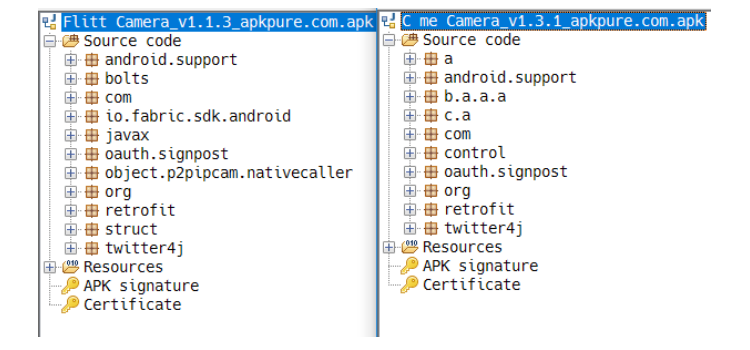
\includegraphics[width=\linewidth]{figures/apk-comparison}
  \caption{Comparison of the APK structures for both in-scope drones}
  \label{fig:apk-comparison}
\end{figure}

\vspace{1cm}
While trying to decompile the applications, we faced two major problems :

\begin{enumerate}
  \item Some parts of the code couldn’t be decompiled
  \item Key parts of the code were obfuscated
\end{enumerate}

\paragraph{Decompilation failures} Java is compiled into an intermediate form, JVM bytecode, which is closer (more similar) to the source than assembly. In particular, \texttt{.class} files include metadata for class names, method names, field and parameter types, etc... All a Java decompiler needs to do is look at the instructions in each method body, and turn them into the appropriate syntactic constructs.

Unfortunately, sometimes it happens that some decompilers fail to reverse parts of the code, especially when anti-debugging measures were used at compilation \cite{anti-debugging}, and the only solution for that -- except coding our own decompiler which is not the intent of this work -- is to find one that does it successfully. We tired to do so with other tools but couldn’t be a hundred percent successful, so we had to work with some portion of the code remaining as shown in the figure.

\begin{figure}[H]
  \centering
  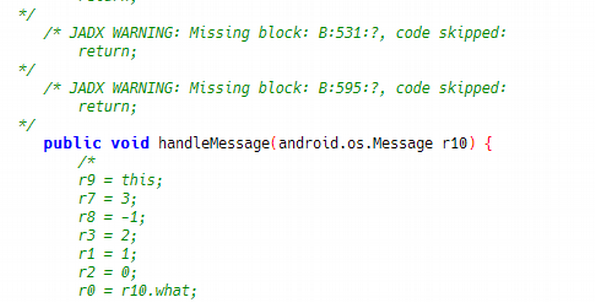
\includegraphics[width=.5\linewidth]{figures/jadx-decompilation-error}
  \caption{Jadx decompilation error example, possibly due to anti-debugging}
\end{figure}

\paragraph{Code obfuscation} There are many ways to obfuscate a source code \cite{code-obfuscation}, and in this case it consists in systematically replacing all the names of classes, methods and variables by single letters. This method was only used on parts of the code, which probably means that some libraries were open source and used as such and others were obviously developed by the manufacturer and protected with obfuscation.

In our case, this represented thousands of single characters making the code completely unreadable. Fortunately, Jadx includes a deobfuscator tool and after using it on the code, most of it was revealed.

\begin{figure}[H]
  \centering
  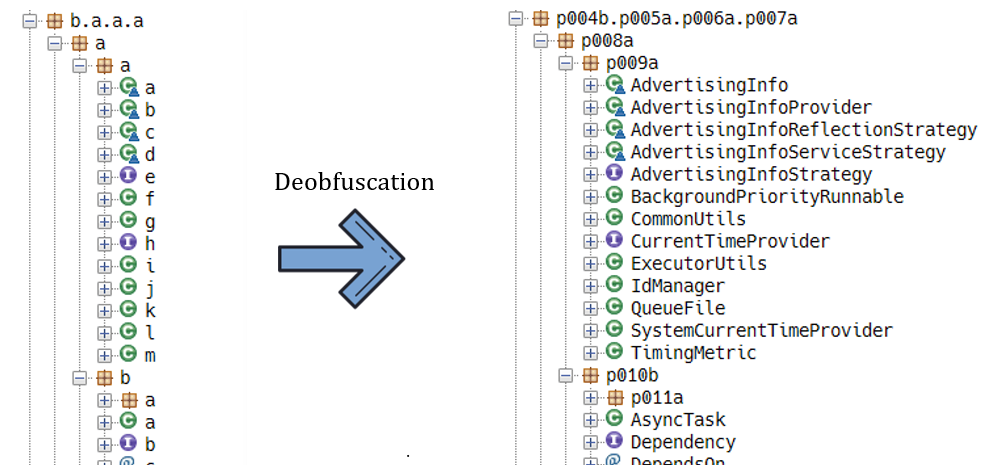
\includegraphics[width=.8\linewidth]{figures/apk-source-deobfuscation}
  \caption{Jadx code deobfuscation, before (on the left) and after (on the right)}
\end{figure}

From there, our objectives were threefold :

\begin{enumerate}
  \item Find default credentials
  \item Understand the fly control/communication protocol
  \item Identify key commands
\end{enumerate}

\paragraph{Default credentials} Unfortunately, nothing to be found here concerning the Flitt, so it appears that the application doesn’t use the Telnet feature. Therefore, we can ask ourselves why the telnet port is open on the drone ! We were more successful with the C-me, since the credentials for the FTP connection were hard-coded in the software. This means that they are similar for every drone.

\begin{figure}[H]
  \centering
  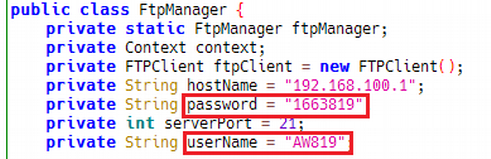
\includegraphics[width=.5\linewidth]{figures/apk-source-with-password}
  \caption{Cleartext username and password hardcoded in the source code}
\end{figure}

\paragraph{Fly control protocol} In this case, both codes were identical in their logic, and having two rather similar applications to work on proved to be rather useful. Indeed, the obfuscation was not always the same in both codes and thus we could use parts of each side in order to try to understand how the protocol was designed and what is being send as commands.

From there, a long process of following variables and trying to understand all the chain of actions that follow each other from the moment when the user clicks on a command on his smartphone and the one when the command is sent to the drone.

The programming is very generic with a high level of abstraction, resulting in a high number of classes and interfaces. Combined with the obfuscation, it is almost impossible to describe the entire process which is triggered when a command is sent clearly and it wouldn’t be much informative.

Nevertheless, the general idea is that there is a main activity, named \texttt{H264Activity}, that corresponds to the screenshot displayed in Subsection \ref{subsec:cme-selfie-drone} and allows the user to send all the control commands from one single point in the program. This obviously makes sense: it wouldn’t be practical for the user to switch between screen in order to navigate the drone. This results in a monster class that contains more than six thousand lines, and unfortunately, a rather big part of it was not successfully decompiled.

From there, the \texttt{H264Activity} calls (through a long succession of interfaces and generic classes) the \texttt{FlyControlThread} which, as indicated by its name, creates a threat responsible to handle the control command.

Before being sent, a \acrfull{crc} is calculated in order to be able to check the communication. \acrshort{crc} is a checksum for detecting transmission or transfer errors by adding, combining and comparing redundant data, obtained through a hashing procedure. The \acrshort{crc}'s are evaluated (sampled) before and after the transmission or transfer, and compared to ensure that the data is probably the same (probably only because not all errors can be detected). The most used \acrshort{crc} calculations are designed to always be able to detect errors of certain types, such as those due for example to interference during transmission.

Finally, the \texttt{FlyControlThread} transmits the command to be sent to the \texttt{UdpControlClient} class that handles the actual transmission. This is done through multiple calls between obfuscated classes, hence the term \textit{calls chain} in Figure \ref{fig:apk-class-interactions}.

\begin{figure}[H]
  \centering
  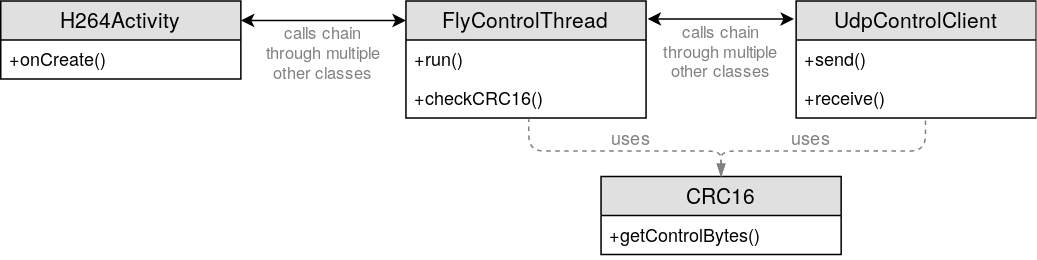
\includegraphics[width=.85\linewidth]{figures/apk-class-interactions}
  \caption{Classes interactions overview (non-UML) for transmitting a command to the drone}
  \label{fig:apk-class-interactions}
\end{figure}

It was unfortunately impossible to forge commands based on the information gathered from this code since the \acrshort{crc} computation used too many variables, some of them coming from parts of the code that weren’t successfully decompiled. We finally stopped to try to do it since it was becoming too time-consuming compared to what could be achieved.

\paragraph{Key control commands} By looking deep into the source code, we were also able to identify a class Config that contained only one long enumeration with what look like a list of configuration commands that can possibly be sent to the drone.

There were in total 75 different commands such as :

\begin{center}
\rowcolors{2}{gray!25}{white}
  \begin{tabular}{C{7cm}L{7cm}}
  \rowcolor{gray!50}
  \hf{7cm}{Name} & \hf{7cm}{Description} \\
  \texttt{CMD\_REQ\_SYS\_PARAM\_GET} & Get a system parameter \\
  \texttt{CMD\_REQ\_DATE\_TIME\_SET} & Set the date and time \\
  \texttt{CMD\_REQ\_PWR\_OFF} & Power off the drone \\
  \texttt{CMD\_REQ\_DEL\_ALL\_FILE} & Delete all files \\
  \texttt{CMD\_REQ\_NET\_DISCONN} & Kick the device connected from the \acrshort{ap} \\
  \texttt{CMD\_REQ\_NET\_SSID} & Change \acrshort{ap}'s \acrshort{ssid} \\
  \texttt{CMD\_REQ\_NET\_PASSWORD} & Change \acrshort{ap}'s password \\
  \texttt{CMD\_REQ\_FACTORY\_RESTORE\_SET} & Set the drone back to its factory defaults \\
  \texttt{CMD\_REQ\_FIRMWARE\_UPDATE} & Trigger firmware update \\
  \end{tabular}
\end{center}

These will reveal to be extremely handy, as it will be shown in Chapter \ref{exploits}.

\subsection{Traffic capture}\label{subsec:traffic-capture}

\begin{warning}
In order to use efficiently Aircrack-ng (see Subsection \ref{subsec:tools-and-resources}), all the following operations were carried out on the Kali Linux OS installed in a virtual machine, with the Panda 300Mbps Wireless 802.11n USB Adapter with High Gain Antenna (PAU061) which provided stable WiFi captures.
\end{warning}



\end{chaptercover}
